\section{Data Acquisition}

During data acquisition the subjects will be wearing the instruments presented earlier in \secref{methods:instrumentation}. One Shimmer3 device will be placed on the subjects torso at the chest. The other is placed at the left knee of the subject. 

The FSRs will be placed on the sole of each foot of the subject. One FSR 406 is placed under the heel and two FSR 402 sensors are placed under the front of the foot at the lateral and medial part of the anterior eminence of the sole. One Arduino Uno will be placed at the back of the hip of the subject to handle data collection. Collected data will be stored on an SD card for later analysis with MATLAB. An illustration of device placement on a subject can be seen in \figref{fig:bodySysSetup}. 

%% SENSOR BAIT ALERT:
%jeg har skrevet at vi placere en FSR 406 (den store firkant sensor) under hælen. vi ved allerede at den skal sidde nærmest storetåen, men det kan vi tage med til vores test afsnit og skrive noget i retningen af:
%sensor bait tekst flyttet til test section

\begin{figure}[H]
	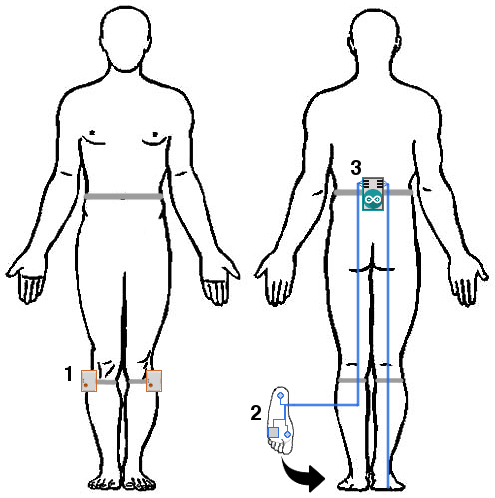
\includegraphics[width=.6\textwidth]{figures/bodySysSetup}
	\caption{The placement of the Shimmer3 IMU devices, Arduino breadboard and FSRs on a test subject.}
	\label{fig:bodySysSetup}  %<--remember LABEL!
\end{figure}

Data acquisition from the Shimmer devices are handled by Bluetooth between the Shimmer devices and MATLAB. Sample frequency over 9000. Data is organized into a matrix, because that is the smart thing to do, when doing things in MATLAB.

A simple but effective graphical user interface (GUI) have been developed to match data from the FSRs to that of the gyroscopes. This manual approach is favourable in this project as it would be more time consuming to develop an algorithm to do it automatically and it also lies beyond the scope for this project. 


we record stuff with the shimmers bluetooth directly to matlab and some jacksticks from the FSR's and save force data to an sd card which we put in matlab and organize it all into one matrix where we can do some math on. 

so far there might not be any filtering of any of the data







